\begin{figure}[htb]
  \begin{center}
    \resizebox{\textwidth}{!}{
      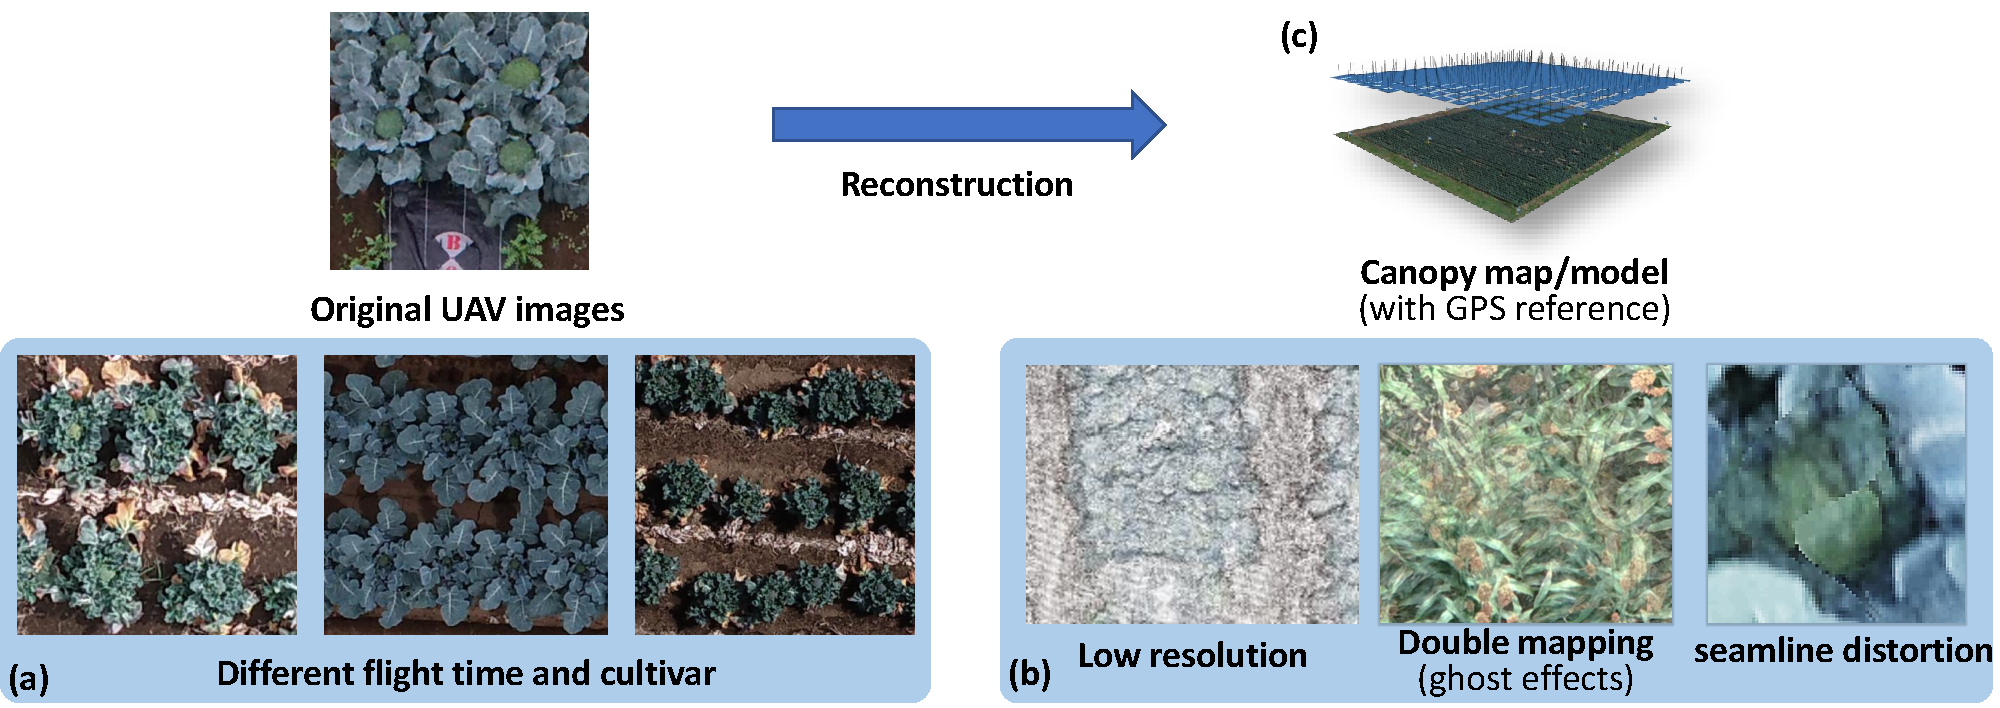
\includegraphics{figures/idp/Fig.1_background.pdf}
    }
  \end{center}
  \caption[Organ-level analysis challenges of UAV-based approach]{
    The main challenges for organ-level analysis on the UAV-based approach. (a) shows the produced canopy 2D map and 3D model often have poor quality, and suffer from double mapping (ghost effect) and seamline distortion. (b) shows the huge differences in time, sunlight, soil condition, growing stage, and cultivars, which makes the image analysis quite difficult. (c) is a figure to show the relationship between raw UAV images and the reconstructed canopy model.
  }
  \label{fig:idp1}
\end{figure}